\documentclass{article}
\usepackage{graphicx}
\usepackage{booktabs}
\usepackage{biblatex}
\addbibresource{citation.bib}

\title{The Effect of Weather Anomalies on Peanut Yield in Florida}
\author{Florian Ullmann}
\date{September 2026}

\begin{document}

\maketitle

\section{Introduction}

\newpage

\section{Background}

\subsection{Agricultural Production in Florida}

Florida is a major agricultural state, with about 44,000 farms managing roughly 9.7 million acres of cropland. The state's farm economy is dominated by crop production: in 2023, approximately 76\% of Florida's \$9.24 billion in cash receipts came from crops, with the balance from livestock. Major commodities include hay and forage, sugarcane, vegetables, and citrus. Peanuts are also an important field crop in Florida. According to the USDA National Agricultural Statistics Service (NASS), Florida farmers planted about 175,000 acres of peanuts in 2025 and harvested 167,000 acres, with an average yield of 3,900 pounds per acre, resulting in approximately 651.3 million pounds of production \cite{FloridaAgricultureOverview}. Florida also typically ranks among the leading U.S. peanut-producing states. In 2022, for example, Florida produced approximately 554 million pounds of peanuts, placing it third among U.S. states, after Georgia and Alabama \cite{PeanutProductionUS}. The importance of peanuts is particularly relevant in the Southeast, which accounts for the majority of U.S. peanut production due in part to its warmer climate and longer growing season \cite{PeanutProductionGuide}.

\subsection{How Peanuts are Produced}

To better understand the factors affecting peanut yields, it is useful to consider the crop's production cycle and its relations to environmental conditions. Peanuts are an annual crop whose growing cycle is closely connected to temperature and water availability. In Florida, runner-type peanuts are generally planted between April 1 and June 1, with planting occurring after the risk of frost has passed and when soil temperatures reach approximately 65--70$^\circ$F \cite{PeanutPlantingDates,FloridaPeanutsIndustry}. A successful crop requires approximately 120--140 frost-free days \cite{FloridaPeanutsIndustry}. 

Approximately 10 days after planting, seedlings emerge from the soil. Unlike many crops, peanuts flower above the ground while their fruit develops below the ground. Yellow flowers generally appear around 40 days after planting. After pollination, the petals fall and the peanut ovary develops into a ``peg,'' which grows downward into the soil, where the peanut pod subsequently develops. Under suitable growing conditions, a single plant can produce approximately 40 or more pods \cite{FloridaPeanutsIndustry}. Depending on the variety and growing conditions, runner peanuts generally mature approximately 135--155 days after planting \cite{PeanutProductionGuide}.

Water availability is particularly important during this production cycle. Peanut plants may require approximately 1.5--2 inches of water per week during kernel development, although requirements vary across growth stages \cite{FloridaPeanutsIndustry}. UF/IFAS identifies approximately 55--100 days after planting, when pod development occurs, as the period of peak water demand, with daily crop water requirements reaching up to approximately 0.20 inches \cite{PeanutProductionGuide}. Insufficient water availability can cause drought stress and reduce yields, while excessive moisture during pod development can increase the risk of soil borne diseases. Water requirements decline as the pods mature \cite{PeanutProductionGuide}.

After maturation, the plants are dug from the soil and placed in windrows with the peanuts facing upward to allow them to dry. At digging, peanuts can contain approximately 25--50\% moisture and are therefore left in the field for several days before being collected by a combine. The combine separates the peanuts from the vines, after which forced warm air can be used to further reduce moisture to an appropriate level for storage \cite{FloridaPeanutsIndustry,PeanutProductionGuide}.

The production cycle illustrates why the timing of weather conditions is important when analyzing peanut yields. Temperature and precipitation can affect the crop differently depending on its stage of development, with water availability being particularly important during pod development. Annual weather measures may hide relevant variation within the growing season. Rather than treating weather as a constant annual characteristic of a county, the  analysis focuses on temperature and precipitation during the period in which peanuts are actually growing. The use of daily weather observations allows these conditions to be aggregated over the relevant growing season and where appropriate, over specific stages of crop development.


\subsection{Existing Research and Motivation}
\label{subsec:existing-research}

Previous research provides evidence that weather conditions during the growing season are important factors for agricultural yields. Eck et al. examine the relationship between growing-season temperature and precipitation anomalies and crop yields for corn, soybeans, cotton, peanuts, and sweet potatoes in the southeastern United States. Using county-level yield data from 1981 to 2018 and growing-season climate anomalies, they find that the relationship between weather conditions and crop yields varies depending on both the crop and the timing of the weather event \cite{InfluceceOfGrowingSeasonTempAnomalies}. Specifically above-normal maximum temperatures during the growing season are associated with significant yield declines, with the largest effects occurring during July and August. For peanuts and sweet potatoes, the authors also find that excessive precipitation during the end of the growing season is detrimental to yields.

These findings are particularly relevant for the empirical approach of this study. They suggest that weather should not necessarily be treated as a constant annual characteristic of a location. Instead, the timing of weather conditions during the crop's growing season may be important for determining agricultural outcomes. For example, annual precipitation could be relatively normal even if a county experiences a period of drought or excessive rainfall during an important stage of peanut development. Therefore, using more detailed weather data makes it possible to construct measures of temperature and precipitation that correspond more closely to the period in which the crop is actually growing.

Research focusing specifically on peanuts provides further evidence that the relationship between weather and yield may be nonlinear. Chalise and Ghimire examine the effects of temperature and precipitation on peanut yields in three agricultural districts in Georgia using historical yield and weather data \cite{PrecipitationOnPeanuts}. Their results indicate that temperature has a positive association with peanut yield over the temperature levels considered in their analysis. However, the effect of precipitation is more complex. Precipitation is associated with higher peanut yields up to a certain level, while additional precipitation beyond this level has a negative effect on yield. This finding is consistent with the agricultural mechanisms discussed previously: insufficient water availability can create water stress, while excessive moisture can create unfavorable conditions for peanut production.

Together, these studies suggest that both the magnitude and timing of weather conditions may be important for peanut production. They also indicate that the relationship between precipitation and yield may not be strictly linear. However, the existing research does not directly examine whether these relationships can be detected in county-level peanut production across Florida over time. This project therefore investigates whether variation in growing-season temperature and precipitation is associated with changes in peanut yields across Florida counties. By combining county-level peanut yield data with daily weather observations, the analysis examines weather conditions during the crop's production cycle rather than relying solely on annual weather averages. This provides the basis for the identification strategy developed in the following sections.

\section{Dataset}

\subsection{Weather Data}

The weather data is obtained from the National Centers for Environmental Information (NCEI) nClimGrid-Daily dataset, which provides gridded, county-level daily maximum, minimum, and average temperature (Tmax, Tmin, Tavg, in $^\circ$C) and daily precipitation (Prcp, in mm) for the United States. Data were downloaded via the NCEI API for all Florida counties, covering the growing season months of April through October for each year from 1991 to 2024, so as to focus on the period during which peanuts are actually in the field rather than on off-season weather.

\subsection{Peanut Yield Data}

Peanut yield data comes from the USDA National Agricultural Statistics Service (NASS) Quick Stats tool:

https://quickstats.nass.usda.gov/\#EC4A8F3C-FF94-3F26-B248-6FDA932248D3
This source provides county-level peanut acres planted, acres harvested, total production, and yield (measured in pounds per acre) for Florida counties. Not every Florida county grows peanuts, and NASS suppresses county-level figures for very small or confidential values, so yield observations are only available for a subset of counties and years.

\subsection{Combined Data}

The unit of observation in the combined dataset is the county-year. For each Florida county and year, the daily growing-season weather observations are aggregated into: mean temperature, mean daily maximum and minimum temperature, total precipitation, the number of ``extreme heat days'' (days with Tmax above 32$^\circ$C, roughly 90$^\circ$F), and the number of ``heavy rain days'' (days with more than 25mm of precipitation, roughly 1 inch). These aggregated weather measures are then merged with the corresponding county-year peanut yield record. Data collection, cleaning, and aggregation were performed in Python using the requests and pandas libraries, with visualizations produced using matplotlib.
\newline After dropping county-years without a recorded yield, the resulting panel contains 420 county-year observations across 22 counties spanning 1991--2024. This panel is unbalanced: only 56.1\% of the county-year cells that would exist if every one of the 22 counties reported a yield in every year from 1991 to 2024 are actually observed, reflecting gaps in NASS county-level reporting over time.

\subsection{Summary Statistics}

Table~\ref{tab:summary-stats} reports summary statistics for peanut yield and the growing-season weather measures across the 420 county-year observations. Average yield is approximately 2,918 lb/acre, with substantial variation (standard deviation of about 741 lb/acre, ranging from 1,205 to 5,143 lb/acre). Growing-season total precipitation also varies considerably across county-years (from 495mm to 1,550mm), while growing-season mean temperature is comparatively stable (23.1$^\circ$C to 26.1$^\circ$C), consistent with Florida's relatively uniform climate across counties and years. The wider spread in precipitation relative to temperature is one motivation for constructing count-based extreme measures, such as extreme heat days, rather than relying on seasonal averages alone.

\begin{table}[h]
\centering
\caption{Summary statistics, county-year panel (N = 420)}
\label{tab:summary-stats}
\begin{tabular}{lrrrr}
\toprule
Variable & Mean & Std. Dev. & Min & Max \\
\midrule
Yield (lb/acre) & 2918.2 & 740.5 & 1205.0 & 5143.0 \\
Total precipitation (mm) & 923.7 & 195.8 & 495.4 & 1550.5 \\
Mean temperature ($^\circ$C) & 24.40 & 0.58 & 23.13 & 26.09 \\
Extreme heat days ($>$32$^\circ$C) & 82.4 & 20.1 & 26 & 135 \\
Heavy rain days ($>$25mm) & 7.8 & 3.2 & 2 & 16 \\
\bottomrule
\end{tabular}
\end{table}

Figure~\ref{fig:hist-yield} shows the distribution of peanut yield across county-years. The distribution is roughly bell-shaped and centered around 2,700--2,900 lb/acre, with a small right tail toward higher-yield county-years.

\begin{figure}[h]
\centering
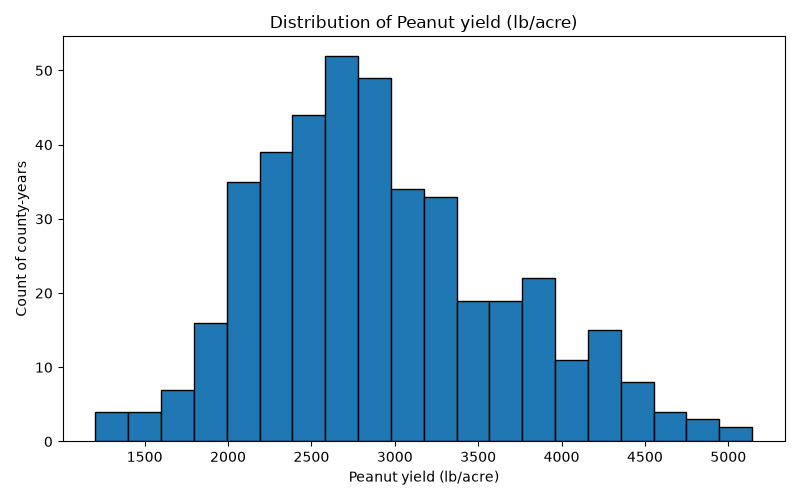
\includegraphics[width=0.7\textwidth]{data/output/figures/hist_yield.png}
\caption{Distribution of peanut yield across county-years}
\label{fig:hist-yield}
\end{figure}

Figure~\ref{fig:boxplot-county} shows yield by county. There is substantial cross-county variation in both the typical yield level and its spread, indicating that county-specific factors (soil type, farming practices, local climate) account for meaningful differences in yield, independent of year-to-year weather variation. This motivates controlling for county-level differences in later analysis.

\begin{figure}[h]
\centering
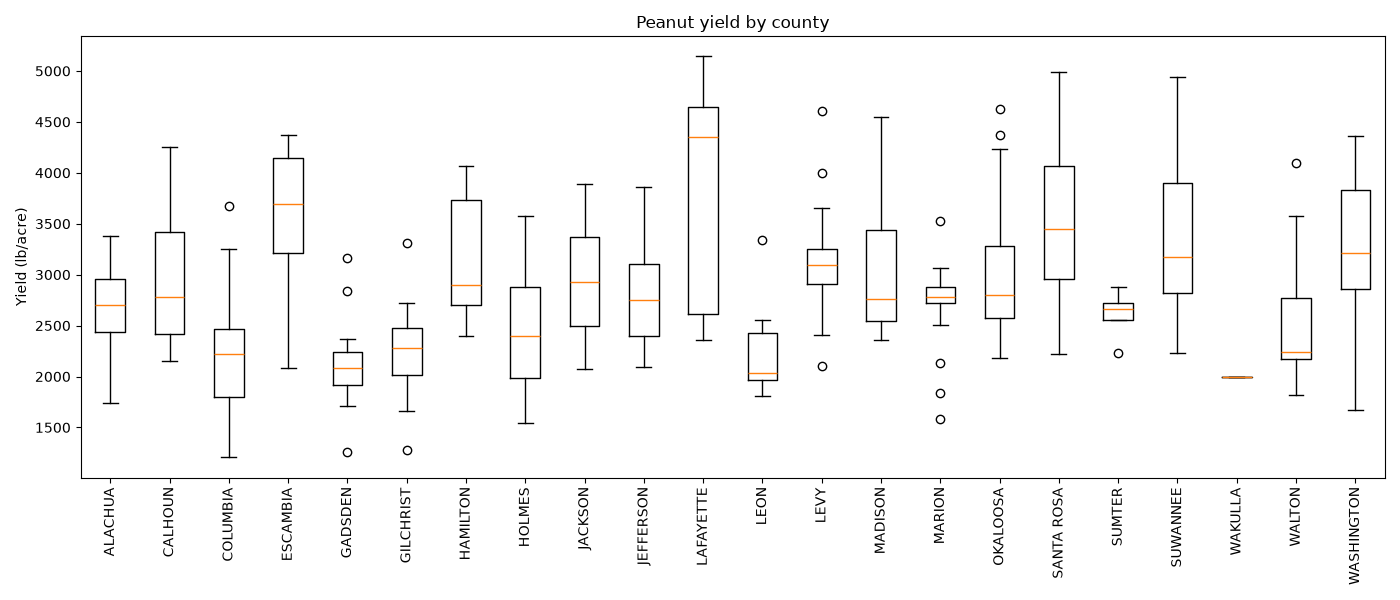
\includegraphics[width=\textwidth]{data/output/figures/boxplot_yield_by_county.png}
\caption{Peanut yield by county}
\label{fig:boxplot-county}
\end{figure}

Finally, Figure~\ref{fig:scatter-prcp} plots yield against growing-season total precipitation. The fitted quadratic trend is close to flat, suggesting that the relationship between yield and precipitation is weak, or at least not well captured by a single growing-season total. This is consistent with the literature reviewed in Section~\ref{subsec:existing-research}, which finds that the timing of precipitation within the growing season, rather than the seasonal total, is what matters most for peanut yield, and motivates the more disaggregated, within-season weather measures to be used in the subsequent analysis.

\begin{figure}[h]
\centering
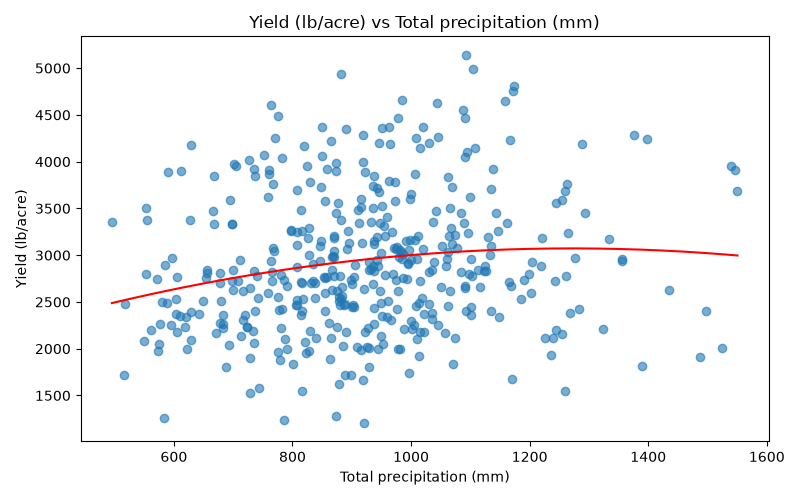
\includegraphics[width=0.7\textwidth]{data/output/figures/scatter_yield_vs_prcp.png}
\caption{Peanut yield vs. growing-season total precipitation, with fitted quadratic trend}
\label{fig:scatter-prcp}
\end{figure}

To check this directly, Figure~\ref{fig:monthly-corr} plots the correlation between yield and each month's weather, computed separately by calendar month rather than pooled over the whole growing season. Both temperature and precipitation are positively correlated with yield from April through August, consistent with favorable early- and mid-season conditions supporting growth. In September and October, however, the pattern reverses: the precipitation correlation turns negative, falling to roughly $-0.15$ in October, while the temperature correlation flattens toward zero. This end-of-season reversal in the precipitation relationship mirrors the finding in Eck et al.~\cite{InfluceceOfGrowingSeasonTempAnomalies} that excess precipitation late in the growing season is specifically detrimental to peanut yield, and it explains why the whole-season total in Figure~\ref{fig:scatter-prcp} appears flat: a positive early-season effect and a negative late-season effect largely cancel out when summed into a single seasonal total. This motivates the use of finer-grained, within-season weather measures --- rather than growing-season totals or averages --- in the identification strategy developed in the next section.

\begin{figure}[h]
\centering
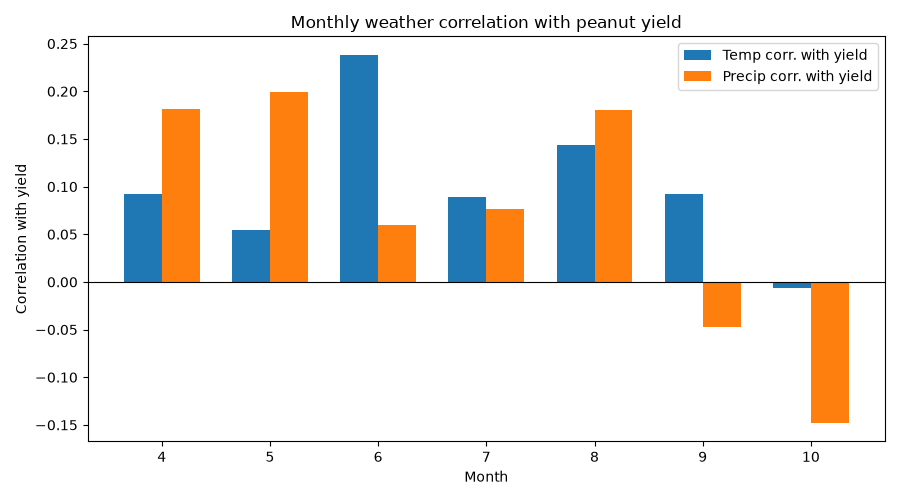
\includegraphics[width=0.8\textwidth]{data/output/figures/monthly_correlation_with_yield.png}
\caption{Correlation of monthly temperature and precipitation with peanut yield, by month}
\label{fig:monthly-corr}
\end{figure}

\newpage

\printbibliography

\end{document}

